%%%%%%%%%%%%%%%%%%%%%%%%%%%%%%%%%%%%%%%%%%%%%%%%%%%%%%%%%%%%%%%%%%%%%%%%%%%%
% AGUtmpl.tex: this template file is for articles formatted with LaTeX2e,
% Modified July 2014
%
% This template includes commands and instructions
% given in the order necessary to produce a final output that will
% satisfy AGU requirements.
%
% PLEASE DO NOT USE YOUR OWN MACROS
% DO NOT USE \newcommand, \renewcommand, or \def.
%
% FOR FIGURES, DO NOT USE \psfrag or \subfigure.
%
%%%%%%%%%%%%%%%%%%%%%%%%%%%%%%%%%%%%%%%%%%%%%%%%%%%%%%%%%%%%%%%%%%%%%%%%%%%%
%
% All questions should be e-mailed to latex@agu.org.
%
%%%%%%%%%%%%%%%%%%%%%%%%%%%%%%%%%%%%%%%%%%%%%%%%%%%%%%%%%%%%%%%%%%%%%%%%%%%%
%
% Step 1: Set the \documentclass
%
% There are two options for article format: two column (default)
% and draft.
%
% PLEASE USE THE DRAFT OPTION TO SUBMIT YOUR PAPERS.
% The draft option produces double spaced output.
%
% Choose the journal abbreviation for the journal you are
% submitting to:

% jgrga JOURNAL OF GEOPHYSICAL RESEARCH
% gbc   GLOBAL BIOCHEMICAL CYCLES
% grl   GEOPHYSICAL RESEARCH LETTERS
% pal   PALEOCEANOGRAPHY
% ras   RADIO SCIENCE
% rog   REVIEWS OF GEOPHYSICS
% tec   TECTONICS
% wrr   WATER RESOURCES RESEARCH
% gc    GEOCHEMISTRY, GEOPHYSICS, GEOSYSTEMS
% sw    SPACE WEATHER
% ms    JAMES
% ef    EARTH'S FUTURE
% ea    EARTH AND SPACE SCIENCE
%
%
%
% (If you are submitting to a journal other than jgrga,
% substitute the initials of the journal for "jgrga" below.)

%\documentclass[draft,jgrga]{agutex2015}
\documentclass[default,jgrga]{agutex2015}
% To create numbered lines:

% If you don't already have lineno.sty, you can download it from
% http://www.ctan.org/tex-archive/macros/latex/contrib/ednotes/
% (or search the internet for lineno.sty ctan), available at TeX Archive Network (CTAN).
% Take care that you always use the latest version.

% To activate the commands, uncomment \usepackage{lineno}
% and \linenumbers*[1]command, below:

% \usepackage{lineno}
% \linenumbers*[1]
%  To add line numbers to lines with equations:
%  \begin{linenomath*}
%  \begin{equation}
%  \end{equation}
%  \end{linenomath*}
%%%%%%%%%%%%%%%%%%%%%%%%%%%%%%%%%%%%%%%%%%%%%%%%%%%%%%%%%%%%%%%%%%%%%%%%%
% Figures and Tables
%
%
% DO NOT USE \psfrag or \subfigure commands.
%
%
%  Uncomment the following command to include .eps files
%  (comment out this line for draft format):
%  \usepackage[dvips]{graphicx}
%
%  Uncomment the following command to allow illustrations to print
%   when using Draft:
%  \setkeys{Gin}{draft=false}
%
% Substitute one of the following for [dvips] above
% if you are using a different driver program and want to
% proof your illustrations on your machine:
%
% [xdvi], [dvipdf], [dvipsone], [dviwindo], [emtex], [dviwin],
% [pctexps],  [pctexwin],  [pctexhp],  [pctex32], [truetex], [tcidvi],
% [oztex], [textures]
%
% See how to enter figures and tables at the end of the article, after
% references.
%
\usepackage{graphicx}
\usepackage{amssymb}
%% ------------------------------------------------------------------------ %%
%
%  ENTER PREAMBLE
%
%% ------------------------------------------------------------------------ %%

% Author names in capital letters:
\authorrunninghead{SALLES ET AL.}

% Shorter version of title entered in capital letters:
\titlerunninghead{High-resolution modeling of Carbonate platform evolution}

%Corresponding author mailing address and e-mail address:
\authoraddr{Corresponding author: Tristan Salles,
School of Geosciences, University of Sydney, Madsen Building, Sydney, NSW 2006, Australia.
(tristan.salles@sydney.edu.au)}

%\authoraddr{Corresponding author: A. B. Smith,
%Department of Hydrology and Water Resources, University of
%Arizona, Harshbarger Building 11, Tucson, AZ 85721, USA.
%(a.b.smith@hwr.arizona.edu)}

\begin{document}

%% ------------------------------------------------------------------------ %%
%
%  TITLE
%
%% ------------------------------------------------------------------------ %%


\title{Exploring millennial responses of reefs to climatic forcing, insights from coupled wave and carbonate growth forward stratigraphic model}
%
% e.g., \title{Terrestrial ring current:
% Origin, formation, and decay $\alpha\beta\Gamma\Delta$}
%

%% ------------------------------------------------------------------------ %%
%
%  AUTHORS AND AFFILIATIONS
%
%% ------------------------------------------------------------------------ %%


%Use \author{\altaffilmark{}} and \altaffiltext{}
\authors{T. Salles\altaffilmark{1}, J. Pall\altaffilmark{1}, J. Webster\altaffilmark{1}, A. Vila-Concejo\altaffilmark{1}, S. Duce\altaffilmark{1}, B. Dechnik\altaffilmark{1}}
\altaffiltext{1}{School of Geosciences, University of Sydney, Sydney, NSW, Australia.}

% \altaffilmark will produce footnote;
% matching \altaffiltext will appear at bottom of page.

% \authors{A. B. Smith,\altaffilmark{1}
% Eric Brown,\altaffilmark{1,2} Rick Williams,\altaffilmark{3}
% John B. McDougall\altaffilmark{4}, and S. Visconti\altaffilmark{5}}

%\altaffiltext{1}{Department of Hydrology and Water Resources,
%University of Arizona, Tucson, Arizona, USA.}

%\altaffiltext{2}{Department of Geography, Ohio State University,
%Columbus, Ohio, USA.}

%\altaffiltext{3}{Department of Space Sciences, University of
%Michigan, Ann Arbor, Michigan, USA.}

%\altaffiltext{4}{Division of Hydrologic Sciences, Desert Research
%Institute, Reno, Nevada, USA.}

%\altaffiltext{5}{Dipartimento di Idraulica, Trasporti ed
%Infrastrutture Civili, Politecnico di Torino, Turin, Italy.}

%% ------------------------------------------------------------------------ %%
%
%  KEYPOINTS
%
%% ------------------------------------------------------------------------ %%

% Key points are 1 to 3 points that the author provides,
% that are 100 characters or less, that are ultimately published
% with the article.
%% for example:
\keypoints{\item Here is the first keypoint.
\item This is the second keypoint.
\item And here is the third keypoint
}


%% ------------------------------------------------------------------------ %%
%
%  ABSTRACT
%
%% ------------------------------------------------------------------------ %%

% >> Do NOT include any \begin...\end commands within
% >> the body of the abstract.

\begin{abstract}
(Type abstract here)
\end{abstract}

%% ------------------------------------------------------------------------ %%
%
%  BEGIN ARTICLE
%
%% ------------------------------------------------------------------------ %%

% The body of the article must start with a \begin{article} command
%
% \end{article} must follow the references section, before the figures
%  and tables.

\begin{article}

%% ------------------------------------------------------------------------ %%
%
%  TEXT
%
%% ------------------------------------------------------------------------ %%

\section{Introduction}
(Article text here.)

\section{Carbonate platform evolution models}

Talk about stratigraphic forward modelling

\section{Model overview}

In this section, a new, deterministic three-dimensional carbonate forward model, pyReef is presented, which simulates reef growth, reef transport and lagoon development based on the coupling between four components: a wave transformation model, a long-term circulation model, a calcareous sand transport model and a carbonate production/disintegration fuzzy logic model (Fig.~\ref{pyreef_sketch}).

\noindent \textbf{pyReef} is an open-source and parallel model mainly written in Python and capable of simulating reef system evolution over time scale of hundreds to thousands of years and over 1 to 10's kilometres scale. The model source code, its associated documentation along with the input files for the examples discussed in this paper are available on Github (http://github.com/pyReef-model). The code is designed to be applied within a variety of environments, from fringing and barrier reefs to carbonate ramps and atolls.

\noindent Below we provide a detailed description of the physical algorithms implemented in pyReef as well as the key assumptions underlying our approach.

\subsection{Extrinsic forcings}

At basin-scale carbonate deposits are strongly controlled by large-scale forcings. Extrinsic processes will affect both the morphology of reef systems and stratigraphy of carbonate depositional sequences by modifying the carbonates production \citep{Hill06}. In pyReef, the following set of external forcing mechanisms could be considered: sea-level oscillations, subsidence/uplift rates, and regional oceanic conditions (\textit{i.e.} sea temperature and acidity).

\begin{figure}
\centering
\noindent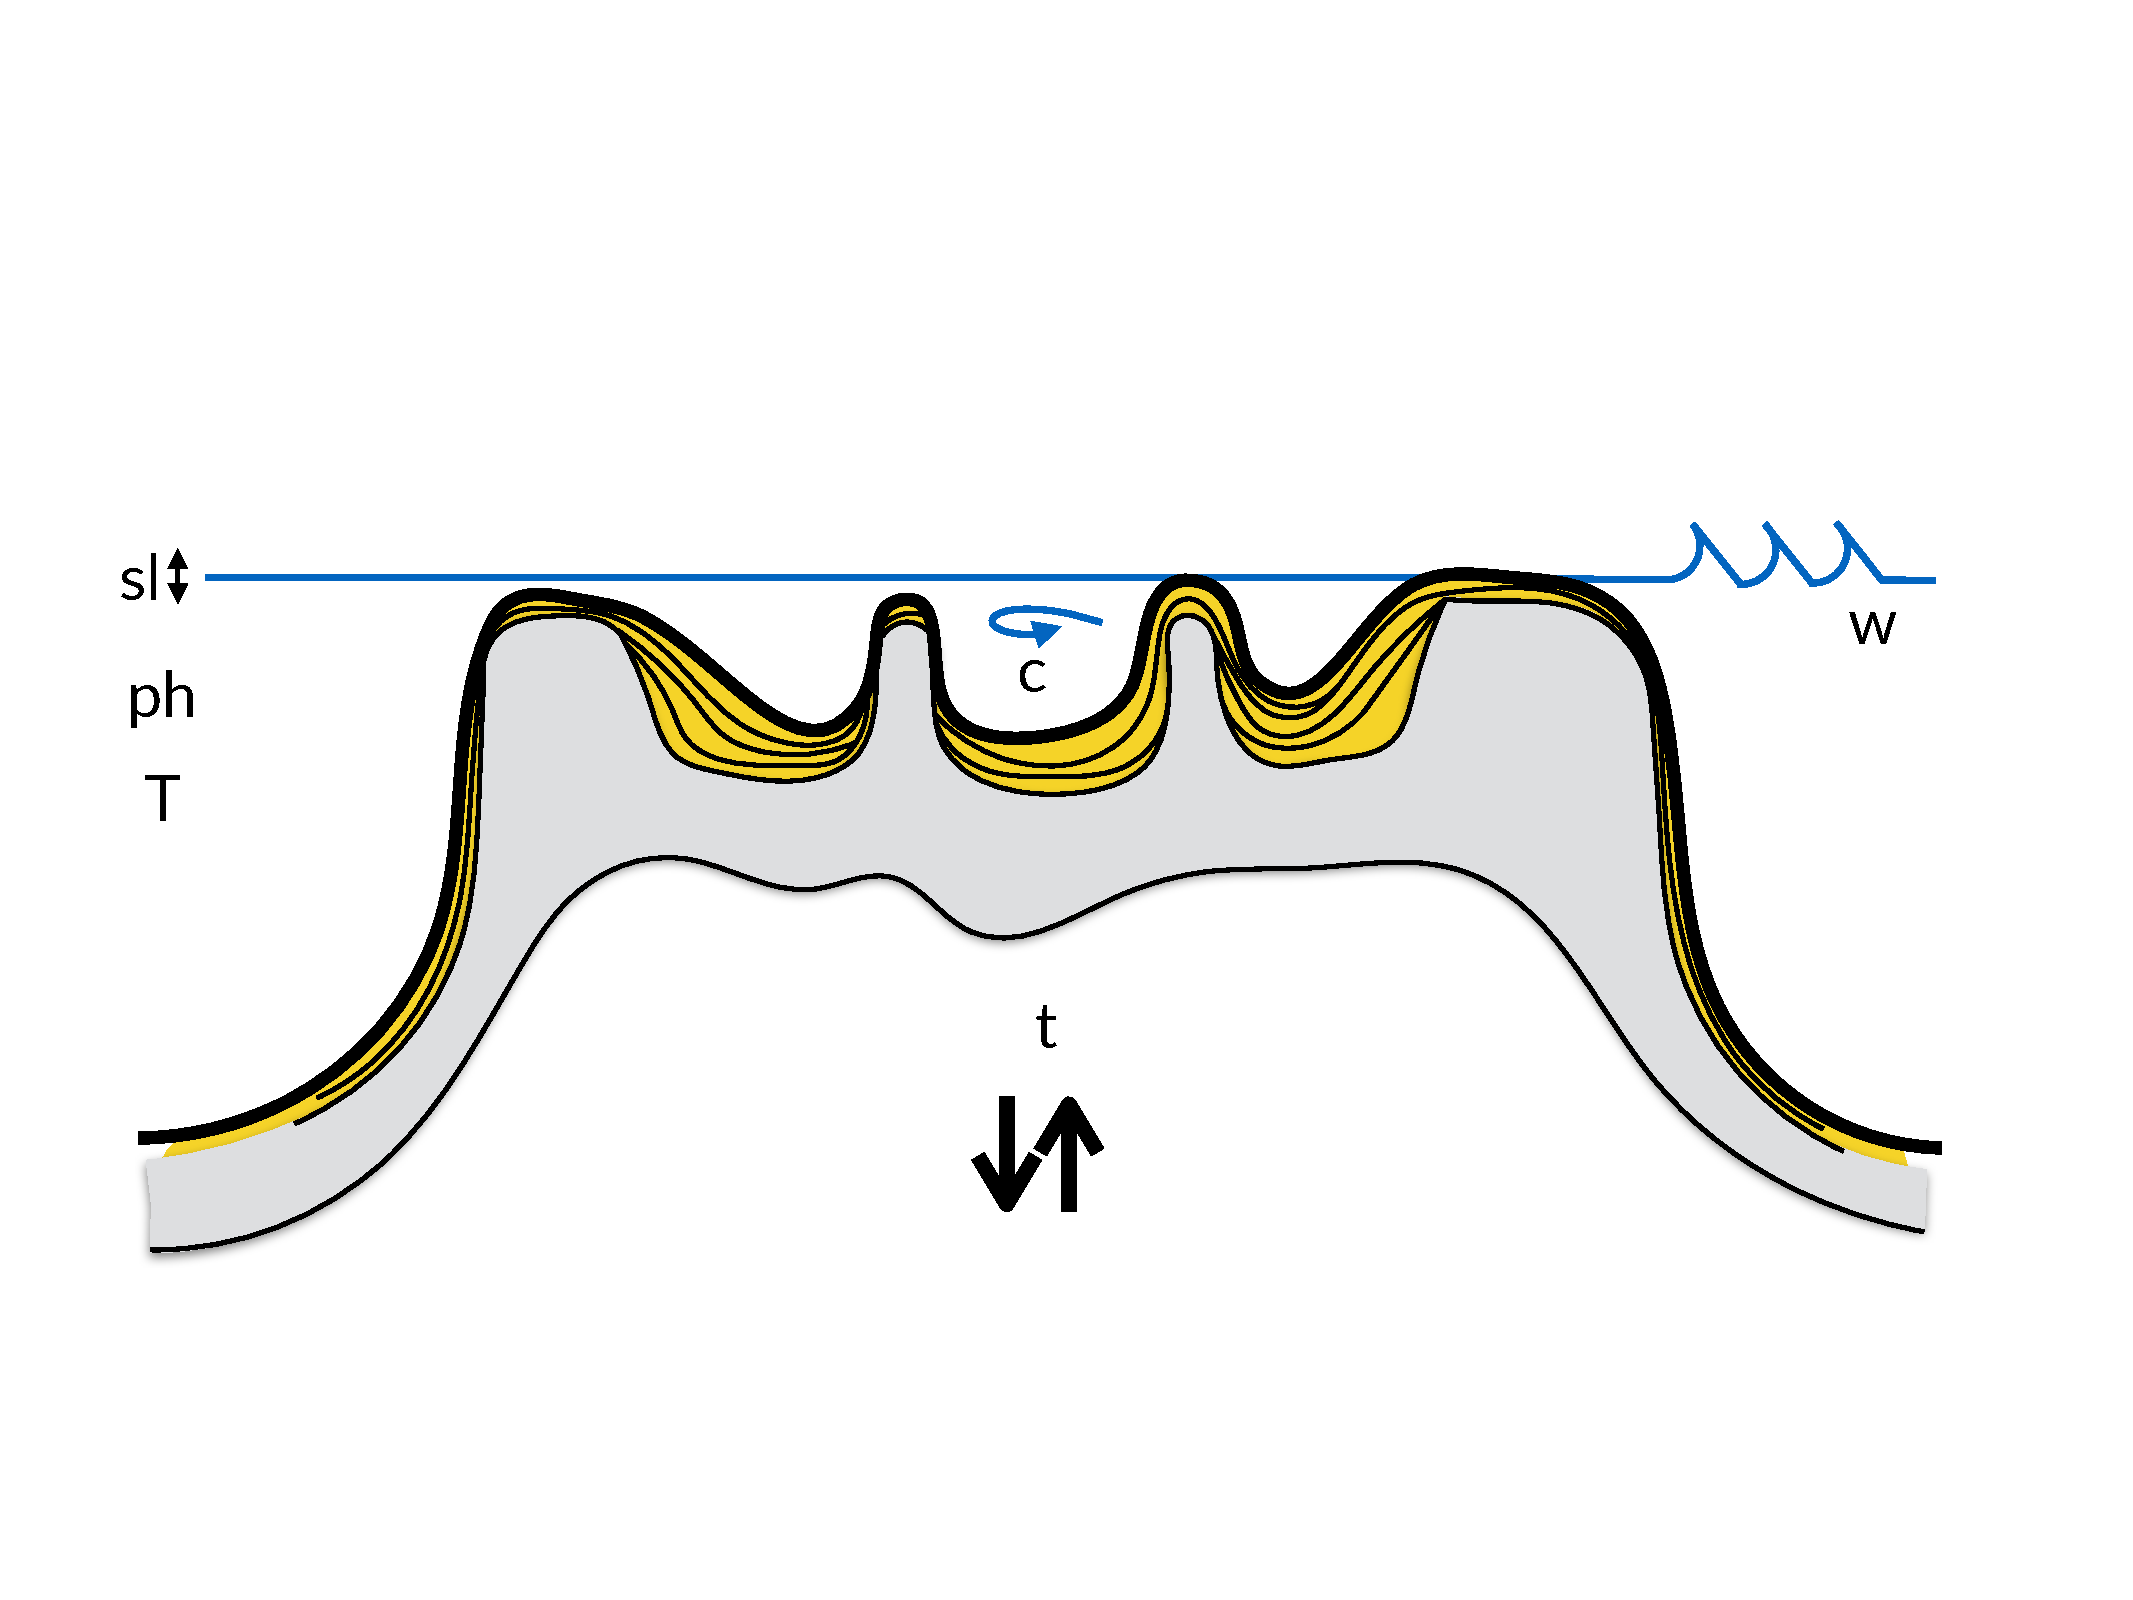
\includegraphics[width=20pc]{figs/fig1.pdf}
\caption{A schematic of 2D coral reef evolution model illustrating the main variables and forces simulated with \textit{pyReef}, where \textbf{w} is wave forcing conditions, \textbf{c} is the long-term ocean circulation, \textbf{sl} is the sea-level, \textbf{t} is the tectonic and \textbf{ph} and \textbf{T} are the ocean's acidity and temperature respectively. The stratigraphic evolution and bed morphology are computes through time and are made of multiple coral assemblages.
}
\label{pyreef_sketch}
\end{figure}

\noindent Accomodation space is a function of relative sea-level changes, which is the sum effect of eustatic sea-level changes, tectonic changes and sediment supply. Several studies have shown that the rates of accretion of coral reefs are largely constrained by changes in accomodation space (\citet{VanWoesik15} or \citet{Roff15} to cite a few). In our model, a sea-level curve can be imported from either a known eustatic curve (\textit{e.g.} such as the ones from \citet{Haq87} or \citet{Miller05}) or directly defined by the user. The tectonic changes are provided as a series of temporal maps. Each map can have variable spatial cumulative displacements making it possible to simulate complex tectonic evolution with both uplift and subsidence conditions. These two forcing mechanisms will directly control the evolution of the hydrodynamic conditions and the associated sediment transport regime as well as the carbonate production described in the following subsections.

\noindent Changing sea surface temperatures and ocean acidification are known to have significant effects across reef systems by controlling the rate of coral reef growth \citep{Shaw12, Andersson13, Zhang13}. In pyReef, long-term regional scale evolution of either ocean's temperature or pH are set by the user as temporal-dependent functions. These functions are then used to control the carbonate production and disintegration as explained in subsection \ref{fuzzy}.

\subsection{Wave transformation}

SWAN, short for \textit{Simulating WAves Nearshore}, is a third-generation, finite-difference, wave model used to predict wave propagation in coastal areas and estuaries. It is governed by the wave action balance equation \citep{Bretherton68, Hasselmann73, Holthuijsen93, Booij99}:

\begin{equation}
 \frac{\partial N}{\partial t}+\nabla_{\vec{x}} \cdot \left[ \left( \vec{c_g} + \vec{U} \right) N \right] + \frac{\partial c_{\theta}N}{\partial \theta} + \frac{\partial c_{\sigma}N}{\partial \sigma} = \frac{S_{tot}}{\sigma}
\end{equation}

\noindent where $N(\vec{x},t,\sigma,\theta)$ is the wave action function of geographical space $\vec{x}$, time $t$, relative frequency $\sigma$ and wave direction $\theta$. $\nabla_{\vec{x}}$ is the gradient operator in space, $\vec{c_g}$ and $\vec{U}$ are the wave group velocity and ambient current vector respectively and $c_{\theta}$, $c_{\sigma}$ is the propagation velocity in $\theta$ and $\sigma$ domain. Finally $S_{tot}$ is the source term which can include wind, whitecapping, surf breaking and bottom friction \citep{Booij99}.

\noindent In our model, shoaling and refraction are accounted for from a series of deep-water wave conditions through time in the absence of wind forcing. Hence to compute wave field generation, the model requires bathymetric conditions and definitions of offshore significant wave height, characteristic period of the energy spectrum, wave direction and associated spreading angle (Fig.~\ref{circfig} panel a and Dir/T distribution plot).

\noindent To evaluate reef responses over several hundreds of years, the approach taken here does not examine temporal evolving wave fields, such as those produced during storm events and relies on SWAN stationary mode. In pyReef, the wave transformation model is generally performed for time intervals varying from $0.5$ to $10$ years. Our aim is to simulate realistic wave fields by imposing a sequence of wave forcing conditions (\textit{e.g.} series of fair-weather and/or storm events). At any given time interval, we define a percentage of activity for each deep-water wave conditions and the bathymetry is used to compute associated wave parameters. Possibility is given to derived these parameters for both low and high tides.

Combined with the climatic forcing described above, two additional wave factors could be adjusted in the model: the breaking parameter and the bottom friction.

\noindent In regions where wave height is close to water depth, wave breaking is an important source of energy dissipation on reefs \citep{Symonds95, Becker14}. This effect is typically approximated with a constant breaking parameter $\gamma_s$ \citep{Symonds95, Vetter10} which values have been calibrated for different reef systems \citep{Apotsos07, Vetter10, Monismith13, Franklin13, Rogers15}.

\noindent The high rugosity of reefs plays a significant role on wave dynamics by increasing the frictional dissipation of wave energy flux \citep{Young89, Lowe05, Lowe15}. This dissipation is usually approximated with a wave roughness friction factor $f_w$ which values have been well constrained for sand grain \citep{Kamphuis75, Grant79, Dean91}. In phase-averaged wave action approach like SWAN, this bottom dissipation is parameterised as a function of wave excursion to bottom roughness scale with a maximum value of 0.3 for $f_w$ \citep{Jonsson66, Madsen88}. Several studies \citep{Nelson96, Lowe05, Lentz15, Rogers15, Monismith15} indicates that this roughness factor can be much higher for reef systems (\textit{i.e.} up to 5.0 for reef platform in the Red Sea \citep{Lentz15}). To better estimate the impact of reef rugosity on frictional dissipation, we have modified the existing formulation for $f_w$ in SWAN and used the proposed parameterisation from \citet{Rogers15} based on  \citet{Swart74}:
\begin{equation}
  \def\arraystretch{1.4}
  f_w=\left\{
    \begin{array}{ll}
      exp\left[ a_1 \left( A_b / k_N \right)^{a_2} + a_3\right], \; A_b/k_N \ge 0.0369 \\
      50, \; A_b/k_N < 0.0369
    \end{array}
  \right.
\end{equation}
\noindent where $A_b$ is the wave excursion distance, $k_N$ is the bottom roughness scale and the coefficients $a_1=$5.213, $a_2=-$0.194, and $a_3=-$5.977 have been set based on \citet{Rogers15}  Palmyra study. Alternate coefficient from \citet{Nielsen92} can also be used ($a_1=$5.5, $a_2=-$0.2, and $a_3=-$6.3). For large values of $A_b/k_N$, this formulation is similar to the one from Madsen et al. [1988] (implemented in SWAN), but extends the parameterisation for lower $A_b/k_N$. In pyReef, the bottom friction is based on the proposed formulation and requires the definition of the bottom roughness scale ($k_N$) which values is generally set to 2-3 times the characteristic diameters of the studied region \citep{Nielsen92, Lowe05, Rogers15}.

\noindent For each forcing conditions, the wave transformation model computes and returns the significant wave height, the mean wave direction and the root-mean-square value of the maxima of the orbital velocity near the bottom (panels c and d in figure \ref{circfig} shows an example of bottom orbital velocity and wave height maps). These parameters are subsequently used to evaluate the long-term hydrodynamic forces active over the simulated region.


\begin{figure*}
\centering
\noindent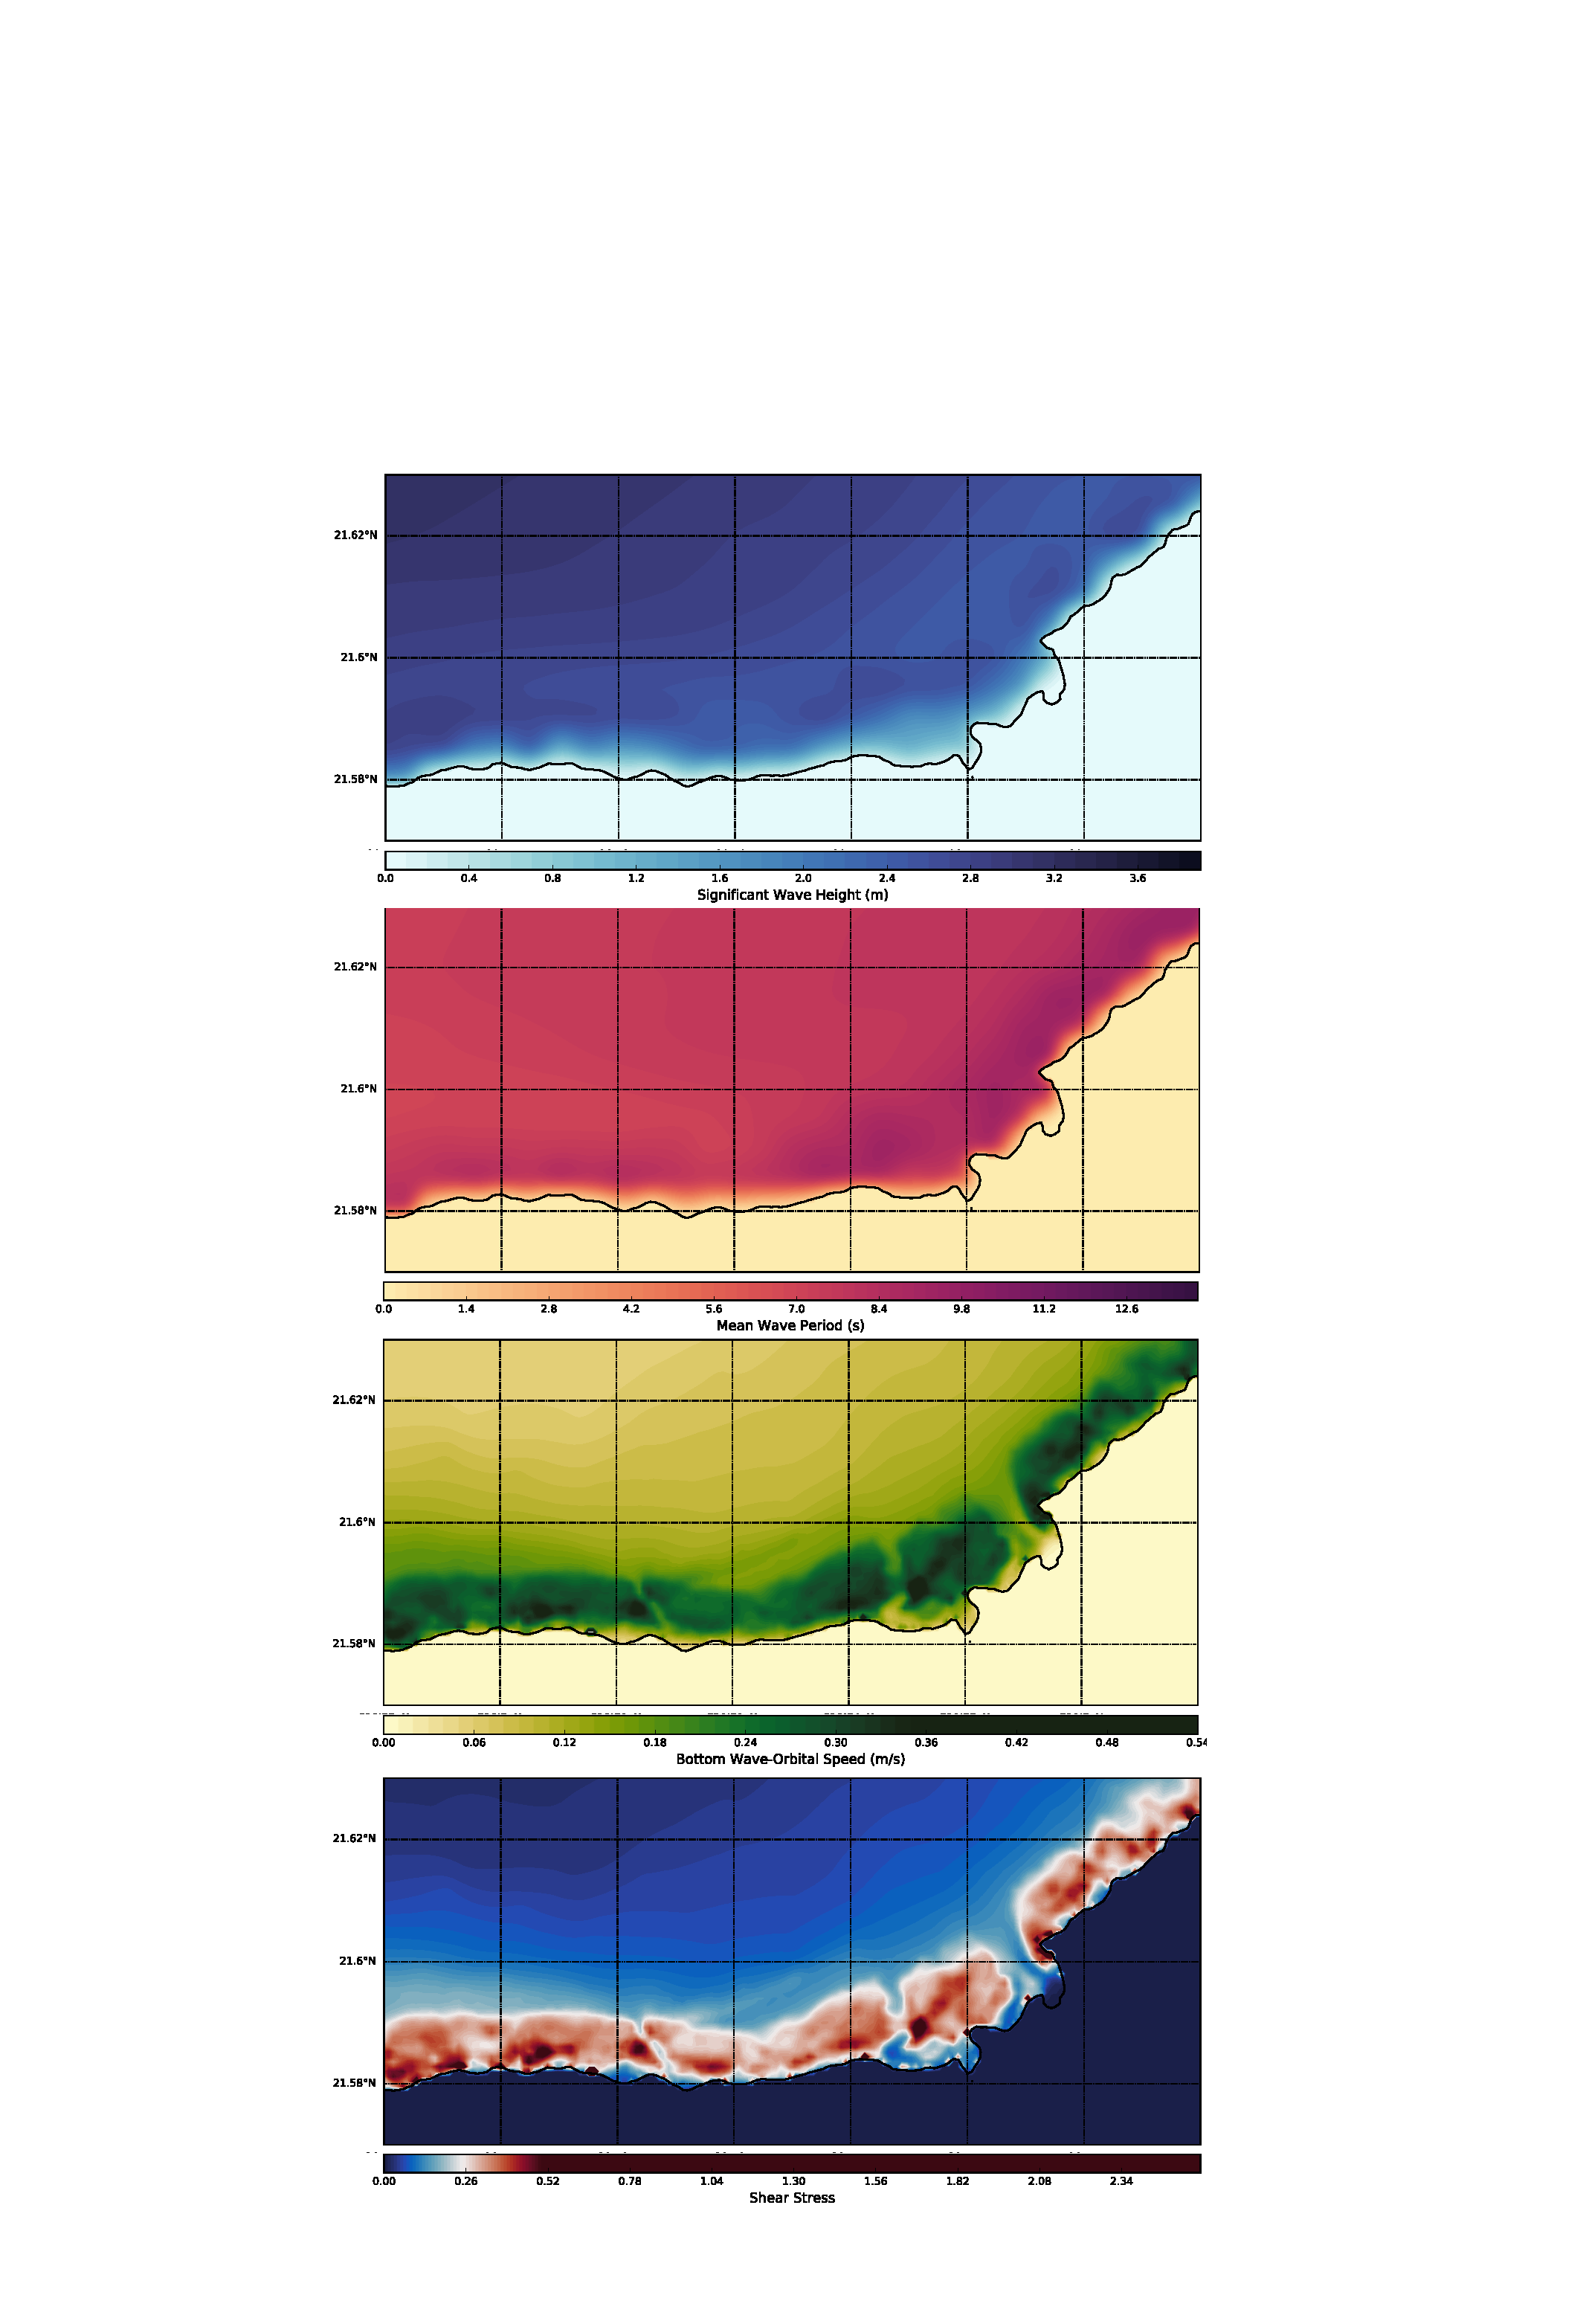
\includegraphics[width=38pc]{figs/fig2.pdf}
\caption{Illustration of sediment transport calculation in pyReef. At time step $t$, a gradient map (\textbf{b}) is first derived from the bathymetry (\textbf{a}). In this example, the circulation is forced by a boundary wave condition characterised by a significant wave height of 4 m, a characteristic period of the energy spectrum of 15 s, and a direction of 150 degrees. The wave transformation model is ran on the bathymetry provided at time $t$ with a reef roughness constant of 0.1 and a wave breaking parameter of 0.66. From the considered boundary conditions, estimates of bottom orbital velocity (\textbf{c}) and wave height (\textbf{d}) are returned and used to compute wave-induced circulation in the area (\textbf{e} and \textbf{g}). The bottom velocity in panel \textbf{e} adds together the longshore and cross-shore components presented in section \ref{seccirc}. The circulation is assumed to be representative of the wave conditions in the area for 5\% of the wave forcing time interval (set to 10\% of the year (roughly 1 month)). From the bottom velocity and main current and wave directions, the model then calculates sediment erosion based on the approach from \citet{Soulsby97}. The erosion and deposition apply only to loose carbonate sands (here only one type of coral assemblages is considered). Erosion takes place on the active layer which is set to 0.25 m and contains 50\% of loose sediments. In addition to circulation-driven transport, a gravity-driven one is implemented and relies on the gradient map (\textbf{b}) and a diffusion coefficient set to 0.1 $\textrm{m}^2\textrm{/yr}$ in this example. The resulting erosion deposition map is presented in panels \textbf{f} and \textbf{h}. From this map both the stratigraphic layers and surface are updated and either a new wave boundary forcing conditions active during the considered time interval is ran or the carbonate growth model is applied.}
\label{circfig}
\end{figure*}

\subsection{Long-term wave-driven circulation}\label{seccirc}

Flow circulation in and around reef platforms depends on the complex interactions between the overlying water motion and the three-dimensional bottom roughness formed by reef organisms. Attempts to numerically simulate flow dynamics around individual coral colonies have been proposed \citep{Kaandorp03, Chang09, Chindapol13} but such models require the flows to be solve down to few millimetres scale and are beyond the scope of our approach. Here we assume that the flow circulation in the reef platform is mainly driven by waves and regional-scale drivers of reefs hydrodynamics such as coastal upwelling or ocean currents are ignored. Numerical studies of wave-driven flow around reef systems commonly use depth-averaged Navier-Stokes equations \citep{Raupach82, Symonds95, Lowe05, Lowe09, Pomeroy12, Taebi11}. In the context of millennial scale reef platform evolution, these methods however are still computationally prohibitive. In pyReef, the proposed method consists in producing \textit{snapshots} of wave-driven circulation distribution resulting from series of deep-water wave scenarios by computing time-averaged cross-shore and longshore currents (Fig.~\ref{circfig} panels e and g).

In nearshore environments, longshore current runs parallel to the shore and is generated by the radiation stresses associated with the breaking process for obliquely incoming waves and by the surplus water which is carried across the breaker zone towards the shoreline \citep{Longuet-Higgins70}. This current affect the transport and transfer of mass (loose carbonate sands, nutrients and carbon) in the nearshore reef waters \citep{Hamner88, Monismith07, Lowe15}. Many empirical formulation of longshore current have been proposed since the initial work from   \citet{Longuet-Higgins64}  \citep{Komar70, Komar75, Galvin87, Reniers97, Ruessink01, Grasmeijer03}. In pyReef, the approach from \citet{Komar75} is used to calculate the longshore current velocity ($\vec{v_l}$) in the middle of the breaking zone:
\begin{equation}
\vec{v_l} = \kappa_l u_{b} cos(\theta) sin(\theta) \vec{k}
\end{equation}
where $u_b$ is the maximum near-bed orbital velocity obtained from SWAN, $\theta$ the angle of incidence of the incoming waves, $\kappa_l$  a scaling parameter and $\vec{k}$ the unit vector parallel to the breaking depth contour. For wave rays approaching the reef at on oblique angle, the component of wave energy flux parallel to the reef shore will drives this longshore velocity. The calculation of the angle of incidence in pyReef is quite straightforward and requires an estimate of wave breaking depth (defined for each wave scenario) and wave direction (obtained from the wave transformation model).

In addition to longshore current, two types of cross-shore velocities are simulated in pyReef. First we estimate the onshore velocity which is essential in predicting the shoreward transport of broken carbonate particles during fair-weather periods  \citep{Elfrink99, Ruessink98}. In our model, we assume a linear dependency between the near-bed orbital velocity and the intensity of this onshore current $\vec{v_o}$:
\begin{equation}
\vec{v_o} = \kappa_o u_b \vec{n}
\end{equation}
with $u_b$ the maximum near-bed orbital velocity, $\vec{n}$ the unit vector parallel to the incoming wave direction and $\kappa_o$ a correction factor. $\kappa_o$ can be derived from local shallow reef water conditions and reflects natural wave skewness and asymmetry which are known to play a central part in cross-shore velocity profile \citep{Grasmeijer03, Crawford03}. The onshore velocity ($\vec{v_o}$) is usually associated to the wave crest and is stronger than the one due to the wave trough \citep{Isobe82, Grasmeijer03}.

During strong wave conditions, a second type of wave-induced cross-shore velocity is defined in pyReef and simulates an offshore-directed steady current referred to as undertow. The time-averaged and depth-averaged undertow velocity $\vec{v_u}$ is derived from the mass flux due to the wave motion and surface roller \citep{Svendsen87}. Under normal incident periodic waves, \citet{Longuet-Higgins75} showed that the depth- and time-averaged undertow velocity is related to the wave's kinetic energy density and phase speed. Assuming  equipartition of kinetic and potential wave energy, the total energy density of the wave is approximately \citep{Svendsen84}:
\begin{equation}
E_w = \frac{1}{8} \rho g H^2
\end{equation}
with $\rho$ the ocean density and  $H$ the root-mean-square wave height returned by SWAN. Following \citet{Cox98}, the undertow velocity is assumed to have the following form in our model:
\begin{equation}
\vec{v_u} = - \kappa_u \frac{\sqrt{g h}}{8} \left(\frac{H}{h} \right)^2 \vec{n}
\end{equation}
with $\kappa_u$ an empirical coefficient \citep{Kobayashi98}, $g$ the gravitational acceleration, $h$ the water depth and $\vec{n}$ the unit vector parallel to the incoming wave direction.

\subsection{Calcareous sand transport}

A common feature of many reef systems is the presence of diverse marine communities, including seagrasses, coral reef organisms, sponges and mangroves. Simulating the evolution of these communities involves to resolve the details of their individual transport by waves and currents at fine scale and therefore requires very advanced and computationally expensive numerical models \citep{Lowe16}. The approach proposed here is based on a parametric transport model that consider the main hydrodynamic forces presented in previous section and  relies on coral assemblages rather than individual communinities. Coral assemblages are derived from coral composition and comparison with modern coral zonation. In the Southern Great Barrier Reef, from 22 identified fossil coral species, \citet{Dechnik15} was able to define four main coral assemblages and their palaeoenvironments. In pyReef, multiple coral assemblages can be defined and we assume that each assemblage is made of hard and loose corals. The hard coral (\textit{e.g.} living part) can either grow in-situ or be disintegrated in loose particles. Only the loose particles are subject to transport and we assume that these particles can be represented by a unique diameter and density value.

To our knowledge, transport law for calcareous sand based on their hydraulic characteristics has not been proposed yet. It has been recognised \citep{Prager96, Day97, Smith04} that variations in the hydraulic properties between siliceous and calcareous sand due to both their shapes and fall velocities lead to different transport behaviors. From flume experiments, \citet{Smith05} shows that transport models designed for siliceous particles might be applied after a correction factor has been introduced. From their experiment, the model of \citet{Engelund67} seems to provide the best fit with their dataset, however they conclude that these corrections are not universally applicable.

\noindent Therefore, in pyReef, we have chosen to build our transport model based on a classical approach. Assuming sediment transport induced by waves and currents, our method is derived from Soulsby and Van Rijn formulation \citep{Soulsby97}. We compute the total load transport rate resulting from the addition of bed load and suspended load for each type of loose carbonate sands initially set by the user. The model also assumes that each of sand particles are perfectly sorted. The method suits well with our approach as it can be applied in a quasi-steady form. An example of erosion deposition for a given long-term circulation representation is illustrated in figure \ref{circfig} panels f and h. The transport rate is defined by:
\begin{equation}
q_t = (A_{sb}+A_{ss}) \bar{v} \left[ \sqrt{\bar{v}^2 + \frac{0.018}{C_D}u_b} - \bar{u_{cr}}\right]^{2.4} (1-1.6 \nabla z)
\end{equation}
\noindent where $\bar{v}$ is the depth-averaged current velocity obtained from the long-term wave driven circulation model defined in previous section, $C_D$ is the drag coefficient (due to current alone) and $\nabla z$ the slope (Fig.~\ref{circfig} panel b). The bed load transport $A_{sb}$ is given by:
\begin{equation}
A_{sb}=\frac{0.005h(d/h)^{1.2}}{(s-1)gd}
\end{equation}
\noindent with $s$ is the relative density of sediments and $d$ is the median grain diameter. The suspended load transport $A_{ss}$ is obtained from the following formula:
\begin{equation}
A_{ss}=\frac{0.012hd_{\star}^{-0.6}}{(s-1)gd}
\end{equation}
\noindent where $d_{\star}$ refers to the dimensionless particle diameter.

\noindent The threshold current velocity of motion ($\bar{u_{cr}}$) is defined by:
\begin{equation}
  \arraycolsep=1.4pt\def\arraystretch{1.4}
  \bar{u_{cr}}=\left\{
    \begin{array}{ll}
      0.19\,d\,^{0.1}\,log_{10}(4h/d), & 0.1 \ge d \ge 0.5 \, \textrm{mm} \\
      8.5\,d\,^{0.6}\,log_{10}(4h/d), & 0.5 \ge d \ge 2. \, \textrm{mm}
    \end{array}
  \right.
\end{equation}

In addition, to the above sediment transport model a multi-lithology non-linear diffusion model has been implemented to simulate secondary gravity-driven transport processes happening over longer temporal scale than wave and current induced ones. Based on \citet{Rivenaes97} and considering $n$ different types of coral assemblages, the following set of nonlinear partial differential equations (PDEs) are used to calculate the proportion of each assemblage $a_k$:
\begin{equation}
  \arraycolsep=2pt\def\arraystretch{2}
    \begin{array}{l}
      \sum_{k=1}^{n} a_k = 1 \\
      \frac{\partial z}{\partial t} = \sum_{k=1}^{n} \frac{1}{c_k} \nabla \cdot ( \kappa_k a_k \nabla z) \\
      d_l \frac{\partial a_k}{\partial t} + a_k \frac{\partial z}{\partial t} = \frac{1}{C_k} \nabla \cdot ( \kappa_k a_k \nabla z)
    \end{array}
\end{equation}

\noindent where $\kappa_k$ denotes the diffusion coefficient for sediment $k$, $c_k$ is the compaction ratio and $d_l$ is a constant representing the thickness of a prescribed top layer, in which sediments are transported. This set of PDEs is solved using a fully explicit schema following the approach from \citet{Clark10}.

To simulate bed morphology and stratigraphic evolution a classical multi-level bed framework tracks the distribution of every coral assemblage through time by layers (\citet{Warner08} and reference therein). In pyReef, each layer stores the bulk properties including thickness and percentage of hard and loose coral assemblages. An active layer at the top of the stratigraphic pile is used to calculate the transport of the calcareous sand from both the wave-current driven and diffusion-based models presented above.

\begin{figure*}
\centering
\noindent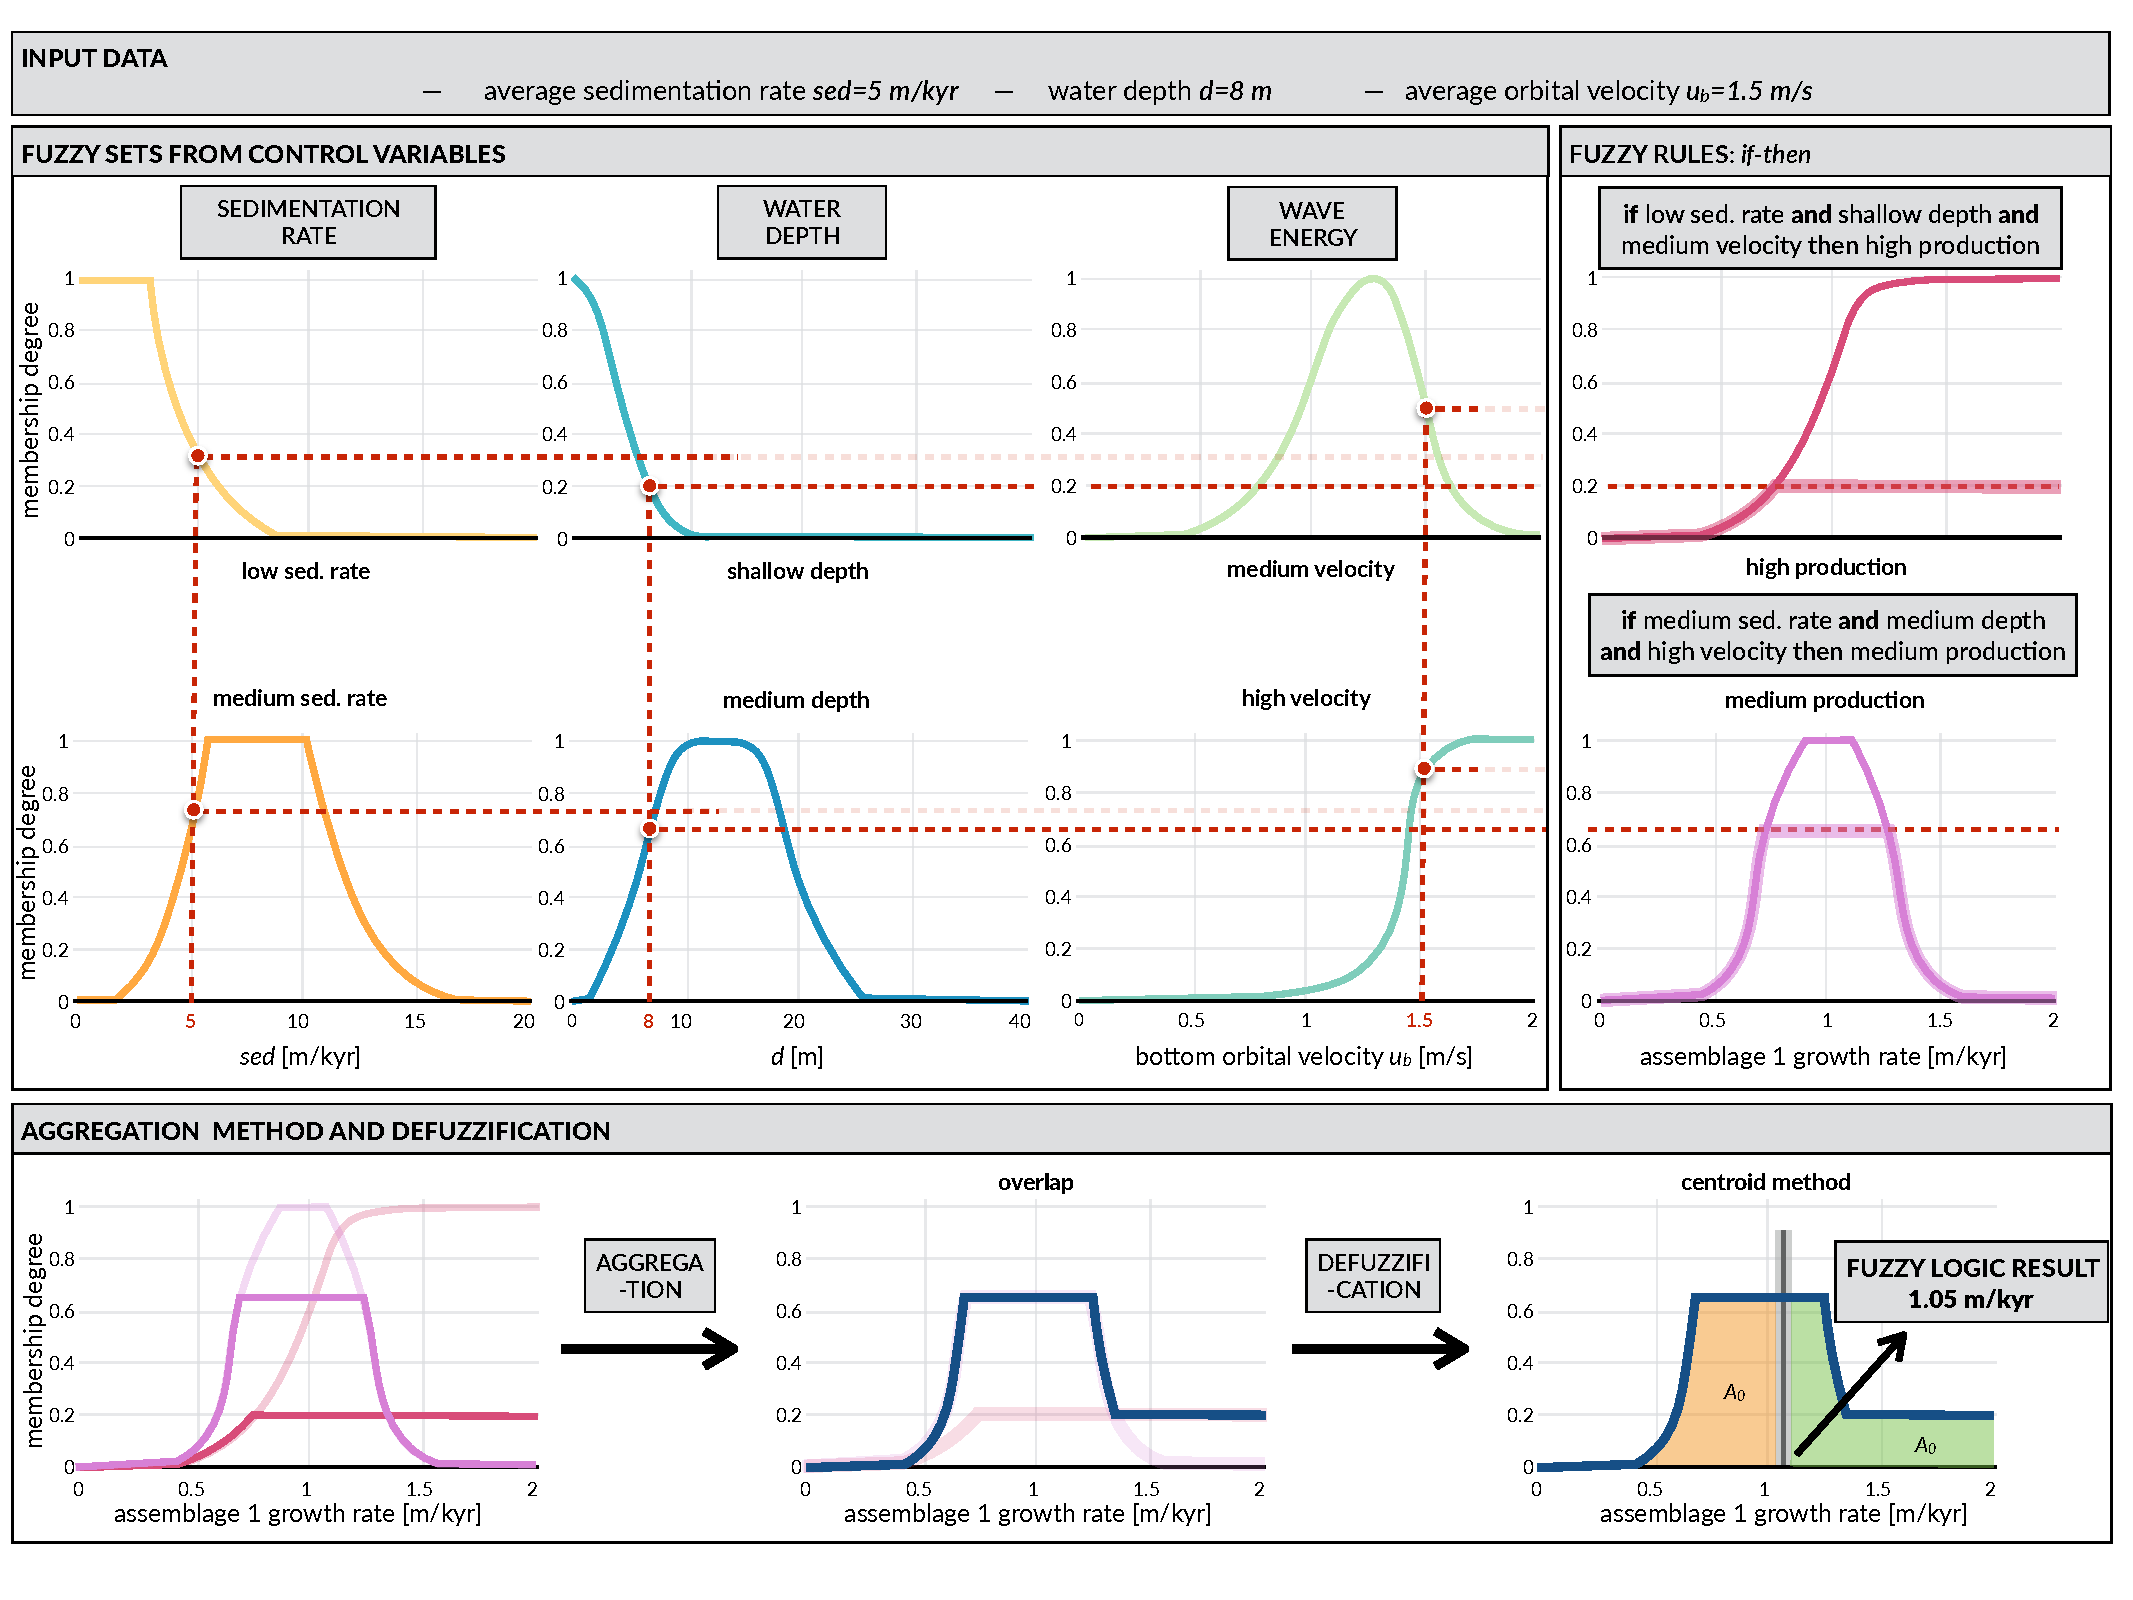
\includegraphics[width=37pc]{figs/fig3.pdf}
\caption{Diagram of fuzzy logic process used in pyReef to evaluate a specific coral assemblage (assemblage 1) growth rate. The approach is illustrated from a point on the carbonate platform with a water depth of 8 m, an average sedimentation rate of 5 m/kyr and an average bottom orbital velocity of 1.5 m/s. The production rate is related to three control variables in this example: the \textit{sedimentation rate}, the \textit{water depth} and the \textit{wave energy}. For each of these variables two membership functions are defined (as an example the water depth is described using the \textit{shallow depth} and \textit{medium depth} functions). The combination of these functions forms a fuzzy set. Two fuzzy rules (based on \textit{if-then} rules) control the production of coral assemblage 1. Each production membership function is then restricted by the minimum (\textit{and} operator) of the membership degree values obtained from combination of the functions active in the considered rule. Aggregation of the truncated production membership functions is done by overlapping the curves and taking the maximum values. Finally the evaluation of the production rate is done through defuzzification by employing the centroid method which returns a \textit{crisp} value of 1.05 m/kyr for the considered point.
}
\label{fuzzyfig}
\end{figure*}

\subsection{Carbonate growth and disintegration}\label{fuzzy}

The organisation of coral reef systems is known to be large and complex and we are still limited in our understanding of their temporal and spatial evolution \citep{Demicco98}. Additionally, most datasets of carbonate systems are often linguistic, context-dependent, and based on measurements with large uncertainties. Conventional deterministic techniques are often enable to address many of the significant variables which affect carbonate productivity \citep{Parcell98}.

Alternative approaches such as fuzzy logic, which is by definition able to cope with these imprecisions \citep{Demicco01, Collin15}, have proven to be a viable alternative to simulate carbonate systems \citep{Salles11, Hattab13}. Fuzzy logic method is able to create logical propositions from qualitative data by using linguistic logic rules and \textit{fuzzy sets} \citep{Nordlund96}. These fuzzy sets are defined with continuous boundaries rather than \textit{crisp} discontinuous ones usually used in conventional approaches \citep{Meesters98}. In depth mathematical theory behind fuzzy logic method can be found in \citet{Zadeh65}, \citet{Zimmerman91} and \citet{Berkan97}.

\noindent Based on a fuzzy logic approach, carbonate system evolution in pyReef is driven entirely by a set of linguistic rules whose variables are fully adjustable. Therefore, the utility and effectiveness of the approach is mostly based on the user's understanding of the modelled carbonate system. The technique is specifically useful to understand how particular variable, in isolation or in combination with other factors, influences carbonate depositional geometries and reef adaptation (Fig. \ref{fuzzyfig}).

In its current form, pyReef employs five types of control variables: depth, wave energy (derived from ocean bottom orbital velocity), sedimentation rate, ocean's temperature and acidity. For each of these variables, one can define a range of fuzzy sets using membership functions \citep{Nordlund99}. A membership function is a curve showing the degree of truth (\textit{i.e.} ranging between 0 and 1) of membership in a particular fuzzy set (Fig. \ref{fuzzyfig}). In pyReef, these curves can be simple triangles, trapezoids, bell-shaped curves, or have more complicated shapes as shown in Fig. \ref{fuzzyfig}. Production and/or disintegration of any specific coral assemblage is then computed from a series of fuzzy rules. A fuzzy rule is a logic \textit{if-then} rule defined from the fuzzy sets \citep{Demicco01}. In our model, the combination of the fuzzy sets in each fuzzy rule is restricted to the \textit{and} operator. The amalgamation of competing fuzzy rules is usually referred to as a fuzzy system. Summation of multiple rules from the fuzzy system by truncation of the membership functions produces a new fuzzy answer in the form of a new membership set (Fig. \ref{fuzzyfig}). The last step consists in computing a single number for this fuzzy set through \textit{defuzzification} \citep{Zadeh65}. In pyReef, the centroid (center of gravity) for the area below the membership set is taken as the \textit{defuzzified} output value.
\\
\\
Coupling of the wave transformation approach (SWAN) with the long-term circulation and sediment transport models and with the fuzzy logic technique presented above allow for numerical analysis of carbonate platforms evolution, stratigraphic architecture reconstruction and provides a numerical framework to quantitatively assess reef system responses to climatic forcing over millennial scales.

\section{Models setup}


\section{Results}

impact of storms on carbonate evolution (model with fair weather and model with 1 storm and after 2 storms)

impact of sea-level change and thermal subsidence

impact of change in pH and ocean temperature

\section{Discussion}


\section{Conclusions}

%%% End of body of article:

%%%%%%%%%%%%%%%%%%%%%%%%%%%%%%%%
%% Optional Appendix goes here
%
% \appendix resets counters and redefines section heads
% but doesn't print anything.
% After typing \appendix
%
%\section{Here Is Appendix Title}
% will show
% Appendix A: Here Is Appendix Title
%
%%%%%%%%%%%%%%%%%%%%%%%%%%%%%%%%%%%%%%%%%%%%%%%%%%%%%%%%%%%%%%%%
%
% Optional Glossary or Notation section, goes here
%
%%%%%%%%%%%%%%
% Glossary is only allowed in Reviews of Geophysics
% \section*{Glossary}
% \paragraph{Term}
% Term Definition here
%
%%%%%%%%%%%%%%
% Notation -- End each entry with a period.
% \begin{notation}
% Term & definition.\\
% Second term & second definition.\\
% \end{notation}
%%%%%%%%%%%%%%%%%%%%%%%%%%%%%%%%%%%%%%%%%%%%%%%%%%%%%%%%%%%%%%%%
%
%  ACKNOWLEDGMENTS

\begin{acknowledgments}
(Text here)
\end{acknowledgments}

%% ------------------------------------------------------------------------ %%
%%  REFERENCE LIST AND TEXT CITATIONS
%
% Either type in your references using
% \begin{thebibliography}{}
% \bibitem{}
% Text
% \end{thebibliography}
%
% Or,
%
% If you use BiBTeX for your references, please use the agufull08.bst file (available at % ftp://ftp.agu.org/journals/latex/journals/Manuscript-Preparation/) to produce your .bbl
% file and copy the contents into your paper here.
%
% Follow these steps:
% 1. Run LaTeX on your LaTeX file.
%
% 2. Make sure the bibliography style appears as \bibliographystyle{agufull08}. Run BiBTeX on your LaTeX
% file.
%
% 3. Open the new .bbl file containing the reference list and
%   copy all the contents into your LaTeX file here.
%
% 4. Comment out the old \bibliographystyle and \bibliography commands.
%
% 5. Run LaTeX on your new file before submitting.
%
% AGU does not want a .bib or a .bbl file. Please copy in the contents of your .bbl file here.

\begin{thebibliography}{}

\bibitem[{\textit{Andersson and Gledhill}(2013)}]{Andersson13}
Andersson, A. J., and D. Gledhill (2013), Ocean acidification and coral reefs: effects on breakdown, dissolution, and net ecosystem calcification, \textit{Annu. Rev. Mar. Sci.}, \textit{5}, 321--48.

\bibitem[{\textit{Apotsos et al.}(2007)}]{Apotsos07}
Apotsos, A., B. Raubenheimer, S. Elgar, R. T. Guza, and J. A. Smith (2007), Effects of wave rollers and bottom stress on wave setup, \textit{J. Geophys. Res.}, \textit{112}, C02003, doi:10.1029/2006JC003549.

\bibitem[{\textit{Becker et al.}(2014)}]{Becker14}
Becker, J. M., M. A. Merrifield, and M. Ford (2014), Water level effects on breaking wave setup for Pacific Island fringing reefs, \textit{J. Geophys. Res. Oceans}, \textit{119}, 914--932, doi:10.1002/2013JC009373.

\bibitem[{\textit{Berkan and Trubatch}(1997)}]{Berkan97}
Berkan, R. C., and S. L. Trubatch (1997), Fuzzy Systems Design Principles: Building Fuzzy IF–THEN Rule Bases: Piscataway, N.J., IEEE Press, 496 p.

\bibitem[{\textit{Booij et~al.}(1999)}]{Booij99}
Booij N., R. Ris, and L. Holthuijsen (1999), A third-generation wave model for coastal regions. 1. Model description and validation, \textit{J. Geophys. Res.}, \textit{104},(C4), 7649--7666.

\bibitem[{\textit{Bretherton and Garrett}(1968)}]{Bretherton68}
Bretherton, F., and C. Garrett (1968), Wavetrains in inhomogeneous moving media, \textit{Proc. R. Soc. Lond. Ser. A}, \textit{302}, 529--554; doi:10.1098/rspa.1968.0034.

\bibitem[{\textit{Chang et~al.}(2009)}]{Chang09}
Chang, S., C. Elkins, M. Alley, J. Eaton, and S. G. Monismith (2009), Flow inside a coral colony measured using magnetic
resonance velocimetry, \textit{Limnol. Oceanogr.}, \textit{54}, 1819.

\bibitem[{\textit{Chindapol et~al.}(2013)}]{Chindapol13}
Chindapol N., J. A. Kaandorp, C. Cronemberger, T. Mass, and A. Genin (2013), Modelling growth and form of the scleractinian coral Pocillopora verrucosa and the influence of hydrodynamics, \textit{PLoS Comput. Biol.}, \textit{9}, e1002849

\bibitem[{\textit{Clark et~al.}(2010)}]{Clark10}
Clark, S. R., W. Wei, and X. Cai (2010), Numerical analysis of a dual-sediment transport model applied to Lake Okeechobee, Florida, \textit{in: Proceedings of the 9th International Symposium on Parallel and Distributed Computing, IEEE Computer Society Press}, pp. 189--194.

\bibitem[{\textit{Collin et~al.}(2015)}]{Collin15}
Collin, A., K. Nadaoka, and L. Bernardo (2015), Mapping the Socio-Economic and Ecological Resilience of Japanese Coral Reefscapes across a Decade, \textit{ISPRS Int. J. Geo-Inf.}, \textit{4}, (2), 900--927.

\bibitem[{\textit{Cox and Kobayashi}(1998)}]{Cox98}
Cox, D. T. and N. Kobayashi (1998), Application of an Undertow Model to Irregular Waves on Plane and Barred Beaches, \textit{J. Coast. Res.}, \textit{14}, 4, 1314--1324.

\bibitem[{\textit{Crawford and Hay}(2003)}]{Crawford03}
Crawford, A. M., and A. E. Hay (2003), Wave orbital velocity skewness and linear transition ripple migration: Comparison with weakly nonlinear theory, \textit{J. Geophys. Res.}, \textit{108}, 3091, doi:10.1029/2001JC001254.

\bibitem[{\textit{Dai}(1997)}]{Day97}
Dai, J. (1997), Engineering Characteristics of Tropical Island Beaches. Master's Thesis, Department of Ocean Engineering, University of Hawaii, Honolulu, Hawaii.

\bibitem[{\textit{Dean and Dalrymple}(1991)}]{Dean91}
Dean, R. G., and R. A. Dalrymple (1991), Water wave mechanics for engineers and scientists, \textit{Advanced Series on Ocean Engineering}, vol. 2, World Sci., Hackensack, N. J.

\bibitem[{\textit{Dechnik et al.}(2015)}]{Dechnik15}
Dechnik, B., J. M. Webster, P. J. Davies, J.-C. Braga, and P. J., Reimer (2015), Holocene 'turn-on' and evolution of the Southern Great Barrier Reef: revisiting reef cores from the Capricorn Bunker Group, \textit{Marine Geology}, \textit{363}, 174--190.

\bibitem[{\textit{Demicco}(1998)}]{Demicco98}
Demicco, R. V. (1998), CYCOPATH 2-D, a two-dimensional, forward-model of cyclic sedimentation on carbonate platforms, \textit{Comput. Geosci.}, \textit{24}, 405--423.

\bibitem[{\textit{Demicco and Klir}(2001)}]{Demicco01}
Demicco, R. V., and G. J. Klir (2001), Stratigraphic simulations using fuzzy logic to model sediment dispersal, \textit{J. Petroleum Science and Engineering}, \textit{31}, 135--155.

\bibitem[{\textit{Elfrink et al.}(1999)}]{Elfrink99}
Elfrink, B., K. A. Rakha, R. Deigaard, and I. Br{\o}ker (1999), Effect of near-bed velocity skewness on cross-shore sediment transport,  \textit{Proceedings Coastal Sediments. ASCE, Reston, VA, USA}, pp. 33--47.

\bibitem[{\textit{Engelund and Hansen}(1967)}]{Engelund67}
Engelund, F., and E. Hansen (1967), A Monograph on Sediment Transport. Technisk Forlag, Copenhagen, Denmark.

\bibitem[{\textit{Franklin et al.}(2013)}]{Franklin13}
Franklin, G., I. Marin~o-Tapia, and A. Torres-Freyermuth (2013), Effects of reef roughness on wave setup and surf zone currents, \textit{J. Coastal Res.}, \textit{Special Issue 65}, 2005--2010.

\bibitem[{\textit{Galvin}(1987)}]{Galvin87}
Galvin, C. (1987), The continuity equation for long shore current velocity with breaker angle adjusted for a wave-current interaction, \textit{Coast. Eng.}, \textit{11(2)}, 115--129.

\bibitem[{\textit{Grant and Madsen}(1979)}]{Grant79}
Grant, W. D., and O. S. Madsen (1979), Combined wave and current interaction with a rough bottom, \textit{J. Geophys. Res.}, \textit{84(C4)}, 1797--1808, doi:10.1029/JC084iC04p01797.

\bibitem[{\textit{Grasmeijer and Ruessink}(2003)}]{Grasmeijer03}
Grasmeijer, B. T., and B. G.Ruessink (2003), Modeling of waves and currents in the nearshore: parametric vs. probabilistic approach, \textit{Coastal Engineering}, \textit{49}, 185--207.

\bibitem[{\textit{Hamner and Wolanski}(1988)}]{Hamner88}
Hamner, W., and E. Wolanski (1988), Hydrodynamic forcing functions and biological processes on coral reefs: a status review, \textit{In Proceedings of the 6th International Coral Reef Symposium, Vol. 1: Plenary Addresses and Status Review, ed. JH Choat, D Barnes, MA Borowitzka, JC Coll, PJ Davies, et al.}, pp. 103--13. Townsville, Aust.: Int. Coral Reef Symp. Exec. Comm.
\bibitem[{\textit{Haq et al.}(1987)}]{Haq87}
Haq, B. U., J. Hardenbol, and P. R. Vail (1987), Chronology of fluctuating sea levels since the Triassic (250 million years ago to present), \textit{Science}, \textit{235}, 1156--1167.

\bibitem[{\textit{Hasselmann et al.}(1973)}]{Hasselmann73}
Hasselmann, K., et al. (1973), Measurements of wind-wave growth and swell decay during the Joint North Sea Wave Project (JONSWAP), \textit{Dtsch. HydrogrZ. 2}, Suppl., 1 (A8), 1--95.

\bibitem[{\textit{Hattab et al.}(2013)}]{Hattab13}
Hattab, T., F. Ben Rais Lasram, C. Albouy, C. Sammari, M. S. Romdhane, P. Cury, F. Leprieur, and F. Le Loc'h (2013), The Use of a Predictive Habitat Model and a Fuzzy Logic Approach for Marine Management and Planning, \textit{PLoS ONE}, \textit{8}, (10), e76430. doi:10.1371/journal.pone.0076430

\bibitem[{\textit{Hill}(2006)}]{Hill06}
Hill, J. (2006), Modelling of reefs and shallow marine carbonates, \textit{Ph.D. Thesis, University of Edinburgh}, 174 p.

\bibitem[{\textit{Holthuijsen et~al.}(1993)}]{Holthuijsen93}
Holthuijsen L.~H, N. Booij, and R.~C. Ris (1993), A spectral wave model for the coastal zone, \textit{Proceedings of the 2nd international symposium on ocean wave measurement and analysis}, \textit{New Orleans, LA}, pp. 630--641.

\bibitem[{\textit{Isobe and  Horikawa}(1982)}]{Isobe82}
Isobe, M., and K. Horikawa (1982), Study on water particle velocities of shoaling and breaking waves,  \textit{Coast. Eng. in Japan},  \textit{25}, 109--123.

\bibitem[{\textit{Jonsson}(1966)}]{Jonsson66}
Jonsson, I. G. (1966), Wave boundary layer and friction factors. \textit{Coastal Eng. Conf.}, \textit{1(10)}, 125--148.

\bibitem[{\textit{Kaandorp et al.}(2003)}]{Kaandorp03}
Kaandorp, J.A., E. A. Koopman, P. M. Sloot, R. P. Bak, M. J. Vermeij, and L. E. Lampmann, (2003), Simulation and analysis of flow patterns around the scleractinian coral Madracis mirabilis (Duchassaing and Michelotti), \textit{Philos. Trans. R. Soc. Lond. B 358}, 1551--57

\bibitem[{\textit{Kobayashi et al.}(1998)}]{Kobayashi98}
Kobayashi, N., M. N. Herrman, B. D. Johnson, and M. D. Orzech (1998), Probability distribution of surface elevations in surf and swash zones, \textit{J. Waterway, Port, Coastal, and Ocean Eng.}, \textit{124}, (3), 99--107.

\bibitem[{\textit{Kamphuis}(1975)}]{Kamphuis75}
Kamphuis, J. (1975), Friction factor under oscillatory waves, \textit{J. Waterw. Harbors Coastal Eng. Div. ASCE}, \textit{101}, 135--144.

\bibitem[{\textit{Komar and Inman}(1970)}]{Komar70}
Komar, P. D., and D. L. Inman (1970), Long-shore sand transport on beaches, \textit{J. Geophys. Res.}, \textit{75(30)}, 5914--5927.

\bibitem[{\textit{Komar and Miller}(1975)}]{Komar75}
Komar , P. D., and M. C. Miller (1975),The initiation of oscillatory ripple marks and the development of plane-bed at high shear stresses under waves, \textit{J. Sed. Res.}, \textit{45(3)}, 697--703.

\bibitem[{\textit{Lentz et~al.}(2015)}]{Lentz15}
Lentz, S. J., J. H. Churchill, K. A. Davis, and J. T. Farrar (2015). Surface gravity wave transformation across a platform coral reef in the Red Sea, \textit{J. Geophys. Res.}, doi:10.1002/2015JC011142.

\bibitem[{\textit{Longuet-Higgins}(1970)}]{Longuet-Higgins70}
Longuet-Higgins, M. S., 1970. Longshore currents generated by obliquely incident sea waves, \textit{J. Geophys. Res.}, \textit{75(33)}, 1--35.

\bibitem[{\textit{Longuet-Higgins}(1975)}]{Longuet-Higgins75}
Longuet-Higgins, M.S. (1975), Integral properties of periodic gravity waves of finite amplitude, \textit{Proceedings of the Royal Society of London A}, \textit{342}(1629), 157--174

\bibitem[{\textit{Longuet-Higgins and Stewart}(1964)}]{Longuet-Higgins64}
Longuet-Higgins, M. S., and R. W. Stewart (1964), Radiation stresses in water waves; a physical discussion, with applications, \textit{Deep-Sea Research}, \textit{11}, 529--562.

\bibitem[{\textit{Lowe et~al.}(2005)}]{Lowe05}
Lowe, R. J., J. L. Falter, M. D. Bandet, G. Pawlak, M. J. Atkinson, S. G. Monismith, and J. R. Koseff (2005), Spectral wave dissipation over a barrier reef, \textit{J. Geophys. Res.}, \textit{110}, C04001, doi:10.1029/2004JC002711.

\bibitem[{\textit{Lowe et~al.}(2009)}]{Lowe09}
Lowe, R.J., J. L. Falter, S. G. Monismith SG, and M. J. Atkinson (2009), A numerical study of circulation in a coastal reef-
lagoon system, \textit{J. Geophys. Res.}, \textit{114}, C06022.

\bibitem[{\textit{Lowe and Falter}(2015)}]{Lowe15}
Lowe, R. J., and J. L. Falter (2015), Sediment transport processes within coral reef and vegetated coastal ecosystems: a review, \textit{WAMSI Dredging Science Node, Report Theme 3, Project 3.1.2}, 19 p.

\bibitem[{\textit{Lowe and Ghisalberti}(2016)}]{Lowe16}
Lowe, R. J., and M. Ghisalberti (2016), Oceanic forcing of coral reefs, \textit{Annu. Rev. Mar. Sci.}, \textit{7}, 43--66, doi:10.1146/annurev-marine-010814-015834.

\bibitem[{\textit{Madsen et al.}(1988)}]{Madsen88}
Madsen, O. S., Y. Poon, and H. C. Graber (1988), Spectral wave attenuation by bottom friction: Theory, \textit{Coastal Eng. Conf.}, \textit{1(21)}, 492--504.

\bibitem[{\textit{Meesters et al.}(1998)}]{Meesters98}
Meesters, E. H., R. P. M. Bak, S. Westmacott, M. Ridgley, and S. Dollar (1998), A fuzzy logic model to predict coral reef development under nutrient stress, \textit{Conserv. Biol.}, \textit{12}, 957--965.

\bibitem[{\textit{Miller et al.}(2005)}]{Miller05}
Miller, K. G., M. A. Kominz, J. V. Browning, J. D. Wright, G. S. Mountain, M. E. Katz, P. J. Sugarman, B. S. Cramer, N. Christie-Blick, and S. F. Pekar (2005), The phanerozoic record of global sea-level change, \textit{Science}, \textit{310}, 1293--1298.

\bibitem[{\textit{Monismith}(2007)}]{Monismith07}
Monismith, S. G. (2007), Hydrodynamics of coral reefs, \textit{Annu. Rev. Fluid Mech.}, \textit{39}, 37--55.

\bibitem[{\textit{Monismith et al.}(2013)}]{Monismith13}
Monismith, S. G., L. Herdman, S. Ahmerkamp, and J. Hench (2013), Wave transformation and wave-driven flow across a steep coral reef, \textit{J. Phys. Oceanogr.}, \textit{43}, 1356--1379, doi:10.1175/JPO-D-12-0164.1.

\bibitem[{\textit{Monismith et al.}(2015)}]{Monismith15}
Monismith, S. G., J. S. Rogers, D. Koweek, and R. B. Dunbar (2015), Frictional wave dissipation on a remarkably rough reef, \textit{Geophys. Res. Lett.}, \textit{42}, 4063--4071, doi:10.1002/2015GL063804.

\bibitem[{\textit{Nelson}(1996)}]{Nelson96}
Nelson, R. C. (1996), Hydraulic roughness of coral reef platforms, \textit{Appl. Ocean Res.}, \textit{18(5)}, 265--274.

\bibitem[{\textit{Nielsen}(1992)}]{Nielsen92}
Nielsen, P. (1992), \textit{Coastal Bottom Boundary Layers and Sediment Transport, Advanced Series on Ocean Engineering}, vol. 4, World Sci., Hackensack, N. J.

\bibitem[{\textit{Nordlund}(1996)}]{Nordlund96}
Nordlund, U. (1996), Formalizing geological knowledge—with and example of modeling stratigraphy using fuzzy logic, \textit{J. Sediment. Res.}, \textit{66}, 689--712.

\bibitem[{\textit{Nordlund}(1999)}]{Nordlund99}
Nordlund, U. (1999), FUZZIM: Forward stratigraphic modeling made simple, \textit{Comp. and Geosc.}, \textit{25}, 449--456.

\bibitem[{\textit{Parcell et al.}(1998)}]{Parcell98}
Parcell, W. C., E. A. Mancini, D. J. Benson, H. Chen, and W. Yang (1998), Geological and computer modeling of 2-D and 3-D carbonate lithofacies trends in the Upper Jurassic Oxfordian, Smackover Formation, Northeastern Gulf Coast, \textit{Abstr. Programs - Geol. Soc. Am. Annu. Meet.}, \textit{30}, A338.

\bibitem[{\textit{Pomeroy et al.}(2012)}]{Pomeroy12}
Pomeroy A., R. J. Lowe, G. Symonds, A. van Dongeren,  and C. Moore (2012), The dynamics of infragravity wave transformation over a fringing reef, \textit{J. Geophys. Res.}, \textit{117}, C11022.
\bibitem[{\textit{Prager et al.}(1996)}]{Prager96}
Prager, E. J., J. B. Southard, and E. R. Vivoni-Gallart (1996), Experiments on the entrainment threshold of well-sorted and poorly sorted carbonate sands, \textit{Sedimentology}, \textit{43}, 33--40.

\bibitem[{\textit{Raupach and Shaw}(1982)}]{Raupach82}
Raupach, M. R., and R. H. Shaw (1982), Averaging procedures for flow within vegetation canopies, \textit{Bound. Layer Me-
teorol.}, \textit{22}, 79--90.

\bibitem[{\textit{Reniers and Battjes}(1997)}]{Reniers97}
Reniers, A. J. H. M., and J. A. Battjes, (1997), A laboratory study of long shore currents over barred and non-barred beaches,  \textit{Coast. Eng.}, \textit{30(1-2)}, 1--21.

\bibitem[{\textit{Rivenaes}(1997)}]{Rivenaes97}
Rivenaes, J. C. (1997), Application of a dual-lithology, depth-dependent diffusion equation in stratigraphic simulation, \textit{Basin Research}, \textit{4}, 2, 133--146.

\bibitem[{\textit{Roff el al.}(2015)}]{Roff15}
Roff, G., J.-X. Zhao, and J. Pandolfi (2015), Rapid accretion of inshore reef slopes from the central Great Barrier Reef during the late Holocene, \textit{Geology}, doi:10.1130/G36478.1.

\bibitem[{\textit{Rogers el al.}(2015)}]{Rogers15}
Rogers, J. S., S. G. Monismith, D. A. Koweek, and R. B. Dunbar (2015), Wave dynamics of a Pacific Atoll with high frictional effects, \textit{J. Geophys. Res. Oceans}, \textit{120}, doi:10.1002/ 2015JC011170.

\bibitem[{\textit{Ruessink et al.}(1998)}]{Ruessink98}
Ruessink, B. G., K. T. Houwman, and P. Hoekstra (1998), The systematic contribution of transporting mechanisms to the cross-shore sediment transport in water depth of 3 to 9 m, \textit{Marine Geology}, \textit{152}, 295--324.

\bibitem[{\textit{Ruessink et al.}(2001)}]{Ruessink01}
Ruessink, B. G., J. R. Miles, F. Feddersen, R. T. Guza, and S. Elgar (2001), Modeling the alongshore current on barred beaches.  \textit{J. Geophys. Res.}, \textit{106}, 22451--22464.

\bibitem[{\textit{Salles et al.}(2011)}]{Salles11}
Salles, T., C. Griffiths, C. Dyt, and F. Li (2011), Australian shelf sediment transport responses to climate change-driven ocean perturbations. \textit{Marine Geology}, \textit{282}, (3-4), 268--274.

\bibitem[{\textit{Shaw et al.}(2012)}]{Shaw12}
Shaw, E. C., B. I. McNeil, and B. Tilbrook (2012), Impacts of ocean acidification in naturally variable coral reef flat ecosystems, \textit{J. Geophys. Res.}, \textit{117}, C03038.

\bibitem[{\textit{Smith and Cheung}(2004)}]{Smith04}
Smith, D. A., and K. F. Cheung (2004), Initiation of motion of calcareous sand, \textit{J. Hydraul. Eng., ASCE}, \textit{130}, 467--472.

\bibitem[{\textit{Smith and Cheung}(2005)}]{Smith05}
Smith, D. A., and K. F. Cheung (2005), Transport rate of calcareous sand in unidirectional flow, \textit{Sedimentology}, \textit{52}, 1009–-1020.

\bibitem[{\textit{Soulsby}(1997)}]{Soulsby97}
Soulsby, R. (1997) Dynamics of marine sand: A manual for practical applications. Thomas Telford Publications, London, 249 pp.

\bibitem[{\textit{Symonds et al.}(1995)}]{Symonds95}
Symonds, G., K. P. Black, and I. R. Young (1995), Wave-driven flow over shallow reefs, \textit{J. Geophys. Res.}, \textit{100(C2)}, 2639--2648, doi:10.1029/94JC02736.

\bibitem[{\textit{Svendsen}(1984)}]{Svendsen84}
Svendsen, L. A. (1984), Mass flux and undertow in a surf zone, \textit{Coastal Eng.}, \textit{8}, 247--365.

\bibitem[{\textit{Svendsen et al.}(1987)}]{Svendsen87}
Svendsen, L. A., H. A. Schaffer, and J. B. Hansen (1987), The interaction between the undertow and the boundary layer flow on a beach, \textit{J. Geophys. Res.}, \textit{92}, C11, 11845--11856.

\bibitem[{\textit{Swart}(1974)}]{Swart74}
Swart, D. H. (1974), Offshore sediment transport and equilibrium beach profiles, PhD Dissertation, TU Delft, Delft University of Technology, Delft, Netherlands.

\bibitem[{\textit{Taebi et al.}(2011)}]{Taebi11}
Taebi, S., R. J. Lowe, C. B. Pattiaratchi, G. N. Ivey,  G. Symonds, and R. Brinkman (2011), Nearshore circulation in a
tropical fringing reef system, \textit{J. Geophys. Res.}, \textit{116}, C02016.

\bibitem[{\textit{Van Woesik et al.}(2015)}]{VanWoesik15}
Van Woesik, R., Y. Golbuu, and G. Roff (2015), Keep up or drown: adjustment of western Pacific coral reefs to sea-level rise in the 21st century, \textit{Royal Society Open Science}, \textit{2}, (7), doi:10.1098/rsos.150181.

\bibitem[{\textit{Vetter et al.}(2010)}]{Vetter10}
Vetter, O., J. M. Becker, M. A. Merrifield, A.-C. P\'equignet, J. Aucan, S. J. Boc, and C. E. Pollock (2010), Wave setup over a Pacific Island fringing reef, \textit{J. Geophys. Res.}, \textit{115}, C12066, doi:10.1029/2010JC006455.

\bibitem[{\textit{Warner et al.}(2008)}]{Warner08}
Warner, J. C., C. R. Sherwood, R. P. Signell, C. Harris, and H. G. Arango (2008), Development of a three-dimensional, regional, coupled wave, current, and sediment-transport model, \textit{Computers and Geosciences}, \textit{34}, 1284--1306.

\bibitem[{\textit{Young}(1989)}]{Young89}
Young, I. R. (1989), Wave transformation over coral reefs, \textit{J. Geophys. Res.}, \textit{94(C7)}, 9779--9789, doi:10.1029/JC094iC07p09779.

\bibitem[{\textit{Zadeh}(1965)}]{Zadeh65}
Zadeh, L. A. (1965), Fuzzy sets, \textit{Information and Control}, \textit{8}, 338--353.

\bibitem[{\textit{Zhang et al.}(2013)}]{Zhang13}
Zhang, Z., J. L. Falter, R. L. Lowe, G. Ivey, M. McCulloch (2013), Atmospheric forcing intensifies the effects of regional ocean warming on reef-scale temperature anomalies during a coral bleaching event, \textit{J. Geophys. Res.}, \textit{118}, 4600–16.

\bibitem[{\textit{Zimmerman}(1991)}]{Zimmerman91}
Zimmerman, H. J. (1991), Fuzzy Set Theory and Its Applications: Boston, Kluwer Academic, 399 p.

%\providecommand{\natexlab}[1]{#1}
%\expandafter\ifx\csname urlstyle\endcsname\relax
%  \providecommand{\doi}[1]{doi:\discretionary{}{}{}#1}\else
%  \providecommand{\doi}{doi:\discretionary{}{}{}\begingroup
%  \urlstyle{rm}\Url}\fi
%
%\bibitem[{\textit{Atkinson and Sloan}(1991)}]{AtkinsonSloan}
%Atkinson, K., and I.~Sloan (1991), The numerical solution of first-kind
%  logarithmic-kernel integral equations on smooth open arcs, \textit{Math.
%  Comp.}, \textit{56}(193), 119--139.
%
%\bibitem[{\textit{Colton and Kress}(1983)}]{ColtonKress1}
%Colton, D., and R.~Kress (1983), \textit{Integral Equation Methods in
%  Scattering Theory}, John Wiley, New York.
%
%\bibitem[{\textit{Hsiao et~al.}(1991)\textit{Hsiao, Stephan, and
%  Wendland}}]{StephanHsiao}
%Hsiao, G.~C., E.~P. Stephan, and W.~L. Wendland (1991), On the {D}irichlet
%  problem in elasticity for a domain exterior to an arc, \textit{J. Comput.
%  Appl. Math.}, \textit{34}(1), 1--19.
%
%\bibitem[{\textit{Lu and Ando}(2012)}]{LuAndo}
%Lu, P., and M.~Ando (2012), Difference of scattering geometrical optics
%  components and line integrals of currents in modified edge representation,
%  \textit{Radio Sci.}, \textit{47},  RS3007, \doi{10.1029/2011RS004899}.

\end{thebibliography}

%Reference citation examples:

%...as shown by \textit{Kilby} [2008].
%...as shown by {\textit  {Lewin}} [1976], {\textit  {Carson}} [1986], {\textit  {Bartholdy and Billi}} [2002], and {\textit  {Rinaldi}} [2003].
%...has been shown [\textit{Kilby et al.}, 2008].
%...has been shown [{\textit  {Lewin}}, 1976; {\textit  {Carson}}, 1986; {\textit  {Bartholdy and Billi}}, 2002; {\textit  {Rinaldi}}, 2003].
%...has been shown [e.g., {\textit  {Lewin}}, 1976; {\textit  {Carson}}, 1986; {\textit  {Bartholdy and Billi}}, 2002; {\textit  {Rinaldi}}, 2003].

%...as shown by \citet{jskilby}.
%...as shown by \citet{lewin76}, \citet{carson86}, \citet{bartoldy02}, and \citet{rinaldi03}.
%...has been shown \citep{jskilbye}.
%...has been shown \citep{lewin76,carson86,bartoldy02,rinaldi03}.
%...has been shown \citep [e.g.,][]{lewin76,carson86,bartoldy02,rinaldi03}.
%
% Please use ONLY \citet and \citep for reference citations.
% DO NOT use other cite commands (e.g., \cite, \citeyear, \nocite, \citealp, etc.).

%% ------------------------------------------------------------------------ %%
%
%  END ARTICLE
%
%% ------------------------------------------------------------------------ %%
\end{article}
%
%
%% Enter Figures and Tables here:
%
% DO NOT USE \psfrag or \subfigure commands.
%
% Figure captions go below the figure.
% Table titles go above tables; all other caption information
%  should be placed in footnotes below the table.
%
%----------------
% EXAMPLE FIGURE
%
 %\begin{figure}
 %\noindent\includegraphics[width=20pc]{samplefigure.eps}
 %\caption{Caption text here}
 %\label{figure_label}
 %\end{figure}
%
% ---------------
% EXAMPLE TABLE
%
%\begin{table}
%\caption{Time of the Transition Between Phase 1 and Phase 2\tablenotemark{a}}
%\centering
%\begin{tabular}{l c}
%\hline
% Run  & Time (min)  \\
%\hline
%  $l1$  & 260   \\
%  $l2$  & 300   \\
%  $l3$  & 340   \\
%  $h1$  & 270   \\
%  $h2$  & 250   \\
%  $h3$  & 380   \\
%  $r1$  & 370   \\
%  $r2$  & 390   \\
%\hline
%\end{tabular}
%\tablenotetext{a}{Footnote text here.}
%\end{table}

% See below for how to make sideways figures or tables.

\end{document}

%%%%%%%%%%%%%%%%%%%%%%%%%%%%%%%%%%%%%%%%%%%%%%%%%%%%%%%%%%%%%%%

More Information and Advice:

%% ------------------------------------------------------------------------ %%
%
%  SECTION HEADS
%
%% ------------------------------------------------------------------------ %%

% Capitalize the first letter of each word (except for
% prepositions, conjunctions, and articles that are
% three or fewer letters).

% AGU follows standard outline style; therefore, there cannot be a section 1 without
% a section 2, or a section 2.3.1 without a section 2.3.2.
% Please make sure your section numbers are balanced.
% ---------------
% Level 1 head
%
% Use the \section{} command to identify level 1 heads;
% type the appropriate head wording between the curly
% brackets, as shown below.
%
%An example:
%\section{Level 1 Head: Introduction}
%
% ---------------
% Level 2 head
%
% Use the \subsection{} command to identify level 2 heads.
%An example:
%\subsection{Level 2 Head}
%
% ---------------
% Level 3 head
%
% Use the \subsubsection{} command to identify level 3 heads
%An example:
%\subsubsection{Level 3 Head}
%
%---------------
% Level 4 head
%
% Use the \subsubsubsection{} command to identify level 3 heads
% An example:
%\subsubsubsection{Level 4 Head} An example.
%
%% ------------------------------------------------------------------------ %%
%
%  IN-TEXT LISTS
%
%% ------------------------------------------------------------------------ %%
%
% Do not use bulleted lists; enumerated lists are okay.
% \begin{enumerate}
% \item
% \item
% \item
% \end{enumerate}
%
%% ------------------------------------------------------------------------ %%
%
%  EQUATIONS
%
%% ------------------------------------------------------------------------ %%

% Single-line equations are centered.
% Equation arrays will appear left-aligned.

Math coded inside display math mode \[ ...\]
 will not be numbered, e.g.,:
 \[ x^2=y^2 + z^2\]

 Math coded inside \begin{equation} and \end{equation} will
 be automatically numbered, e.g.,:
 \begin{equation}
 x^2=y^2 + z^2
 \end{equation}

% IF YOU HAVE MULTI-LINE EQUATIONS, PLEASE
% BREAK THE EQUATIONS INTO TWO OR MORE LINES
% OF SINGLE COLUMN WIDTH (20 pc, 8.3 cm)
% using double backslashes (\\).

% To create multiline equations, use the
% \begin{eqnarray} and \end{eqnarray} environment
% as demonstrated below.
\begin{eqnarray}
  x_{1} & = & (x - x_{0}) \cos \Theta \nonumber \\
        && + (y - y_{0}) \sin \Theta  \nonumber \\
  y_{1} & = & -(x - x_{0}) \sin \Theta \nonumber \\
        && + (y - y_{0}) \cos \Theta.
\end{eqnarray}

%If you don't want an equation number, use the star form:
%\begin{eqnarray*}...\end{eqnarray*}

% Break each line at a sign of operation
% (+, -, etc.) if possible, with the sign of operation
% on the new line.

% Indent second and subsequent lines to align with
% the first character following the equal sign on the
% first line.

% Use an \hspace{} command to insert horizontal space
% into your equation if necessary. Place an appropriate
% unit of measure between the curly braces, e.g.
% \hspace{1in}; you may have to experiment to achieve
% the correct amount of space.


%% ------------------------------------------------------------------------ %%
%
%  EQUATION NUMBERING: COUNTER
%
%% ------------------------------------------------------------------------ %%

% You may change equation numbering by resetting
% the equation counter or by explicitly numbering
% an equation.

% To explicitly number an equation, type \eqnum{}
% (with the desired number between the brackets)
% after the \begin{equation} or \begin{eqnarray}
% command.  The \eqnum{} command will affect only
% the equation it appears with; LaTeX will number
% any equations appearing later in the manuscript
% according to the equation counter.
%

% If you have a multiline equation that needs only
% one equation number, use a \nonumber command in
% front of the double backslashes (\\) as shown in
% the multiline equation above.

%% ------------------------------------------------------------------------ %%
%
%  SIDEWAYS FIGURE AND TABLE EXAMPLES
%
%% ------------------------------------------------------------------------ %%
%
% For tables and figures, add \usepackage{rotating} to the paper and add the rotating.sty file to the folder.
% AGU prefers the use of {sidewaystable} over {landscapetable} as it causes fewer problems.
%
% \begin{sidewaysfigure}
% \includegraphics[width=20pc]{samplefigure.eps}
% \caption{caption here}
% \label{label_here}
% \end{sidewaysfigure}
%
%
%
% \begin{sidewaystable}
% \caption{}
% \begin{tabular}
% Table layout here.
% \end{tabular}
% \end{sidewaystable}
%
%
